\documentclass[a4paper]{article}

%% Language and font encodings
\usepackage[french]{babel}
\usepackage[utf8x]{inputenc}
\usepackage[T1]{fontenc}

%% Sets page size and margins
\usepackage[a4paper,top=3cm,bottom=3cm,left=2cm,right=2cm,marginparwidth=2cm]{geometry}

%% Useful packages
\usepackage{amsmath}
\usepackage{graphicx}
\usepackage[colorinlistoftodos]{todonotes}
\usepackage[colorlinks=true, allcolors=black]{hyperref}
\usepackage{fourier-orns}
\usepackage{titlesec}
\usepackage{fancyhdr}
\usepackage{fancyvrb}
\usepackage{float}
\pagestyle{fancy} 
\setcounter{tocdepth}{5}

%% Tikz stuff
\usepackage{tikz}
\usetikzlibrary{calc, arrows}
\tikzstyle{incolore} = [rectangle, rounded corners, draw=black, minimum height=1cm, minimum width=3cm, text width=3cm, text centered]

\usepackage{libertine}
\newcommand{\hsp}{\hspace{20pt}}
\newcommand{\HRule}{\rule{\linewidth}{0.5mm}}

\renewcommand{\headrulewidth}{1pt}
\fancyhead[C]{} 
\fancyhead[L]{}
\fancyhead[R]{\footnotesize{\leftmark}}

\renewcommand{\footrulewidth}{1pt}
\fancyfoot[C]{}
\fancyhead[L]{}
\fancyfoot[R]{\thepage}

\definecolor{Zgris}{rgb}{0.87,0.85,0.85}

\usepackage{eso-pic,graphicx}
\usepackage{xcolor}
\newcommand{\bgimg}[1]
{
    \AddToShipoutPicture
    {
        \put(\LenToUnit{0 cm},\LenToUnit{0 cm})
        {
            \includegraphics[width=\paperwidth,height=\paperheight]{#1}
        }
    }
}
\begin{document}





\begin{titlepage}
    \begin{sffamily}
        \begin{center}
            
\includegraphics[width=5cm]{images/LogoHenallux.PNG}~\\[1.5cm]
            \textsc{\Large Rapport de laboratoire}\\[1.5cm]

            % Title
            \HRule \\[0.4cm]
            { \huge \bfseries Huitième laboratoire : Conversion AN-NA\\[0.4cm] }
            \HRule \\[2cm]

            % Author and supervisor
            \begin{minipage}{0.4\textwidth}
                \begin{flushleft} \large
                    Roumache Grégoire\\
                    Sénéchal Julien\\
                    Robert Alexandre\\
                    Wallemme Maxime\\
                    Kenmeugne Lionel\\
                    Didion Charles
                \end{flushleft}
            \end{minipage}
            \begin{minipage}{0.55\textwidth}
                \begin{flushright} \large
                    Laboratoire de sciences appliquées à l'informatique\\
                    Sécurité des systèmes, technologie de l'informatique\\
                    Hénallux\\
                    Première année, groupe H \\
                    Année académique 2019-2020\\
                \end{flushright}
            \end{minipage}
            \vfill

            % Bottom of the page
            {\large 14 mai 2020}
        \end{center}
    \end{sffamily}
\end{titlepage}







\let\cleardoublepage\clearpage















\section{Introduction}





Le but de ce laboratoire est de comprendre les différents convertisseurs et ce à quoi ils servent (dans quels cas de figure va t’on utiliser un convertisseur ou un autre). On comprend assez vite que s'il faut utiliser un ordinateur, les données doivent être dans un langage informatique compréhensible par la machine et par conséquent au format numérique.

Les questions auxquelles on devra répondre seront de l’ordre "pourquoi celui là plutôt qu’un autre" pour ce qui est des différentes caractéristiques des convertisseurs.

Les critères pris en compte seront des rapports entre prix et performance par rapport à la tâche que l’on cherche à accomplir. En effet, il semble judicieux de choisir un convertisseur le moins coûteux possible tant que les performances de l’instrument sont suffisantes. Il faut également considérer la tension nécessaire et la question de l’unité de mesure choisie pour représenter la valeur. 














\section{Rappels théoriques}










\subsection{Quels sont les différents types de convertisseurs ?}





Il existe deux grand types de convertisseurs, les AN et les NA.
AN signifie Analogique - Numérique. Ces derniers permettent de numériser un signal analogique comme par exemple le son capté par un micro, en un signal numérique. Pour ce faire, on peut utiliser plusieurs types de convertisseurs comme un convertisseur à rampe simple, un sigma delta ou un Flash.

Le convertisseur à rampe simple par exemple fonctionne de la façon suivante. Un générateur de rampe est couplé à un générateur d’horloges, ce qui nous donne un signal contenant les différentes tentions possibles. Ce dernier est alors comparé avec le signal analogue, et quand les tensions sont égales, la valeur est sortie. Ces convertisseurs sont lents et on presque tous été remplacés par des sigma delta.

Dans un convertisseur sigma delta, un comparateur est utilisé pour convertir sur un bit la différence entre le signal d'entrée et le résultat de la conversion (0=plus petit, 1=plus grand). Cette valeur est alors entrée dans un filtre appelé le décimateur, qui somme les échantillons du signal d'entrée. Ça revient à calculer l'intégrale de la différence entre l'entrée et la sortie. Ce qui fait osciller la valeur de l’intégrale autour d’une valeur de référence. Ces convertisseurs ont pour avantage de pouvoir fournir un signal d’une très haute résolution.

Enfin, NA signifie numérique - analogues, les valeurs analogues sont alors générées au fur et à mesure de l’arrivée du signal numérique.










\subsection{Quelle est la différence entre une conversion AN et NA ?}





Tout d'abord, voici la significations de ces acronymes:
\begin{itemize}
    \item La conversion AN (Analogic to Numeric) est la conversion d'un signal analogique, c'est à dire un signal continu, en un signal numérique discret.
    \item La conversion NA (Numeric to Analogic), c'est le contraire, on convertit un signal numérique discret en un signal continu.
\end{itemize}
Sur la figure \ref{fig:conversionANNA}, la conversion AN est la conversion du signal continu noir mesuré en volt, en un signal discret vert qui est une valeur binaire.

\begin{figure}[H]
    \centering
    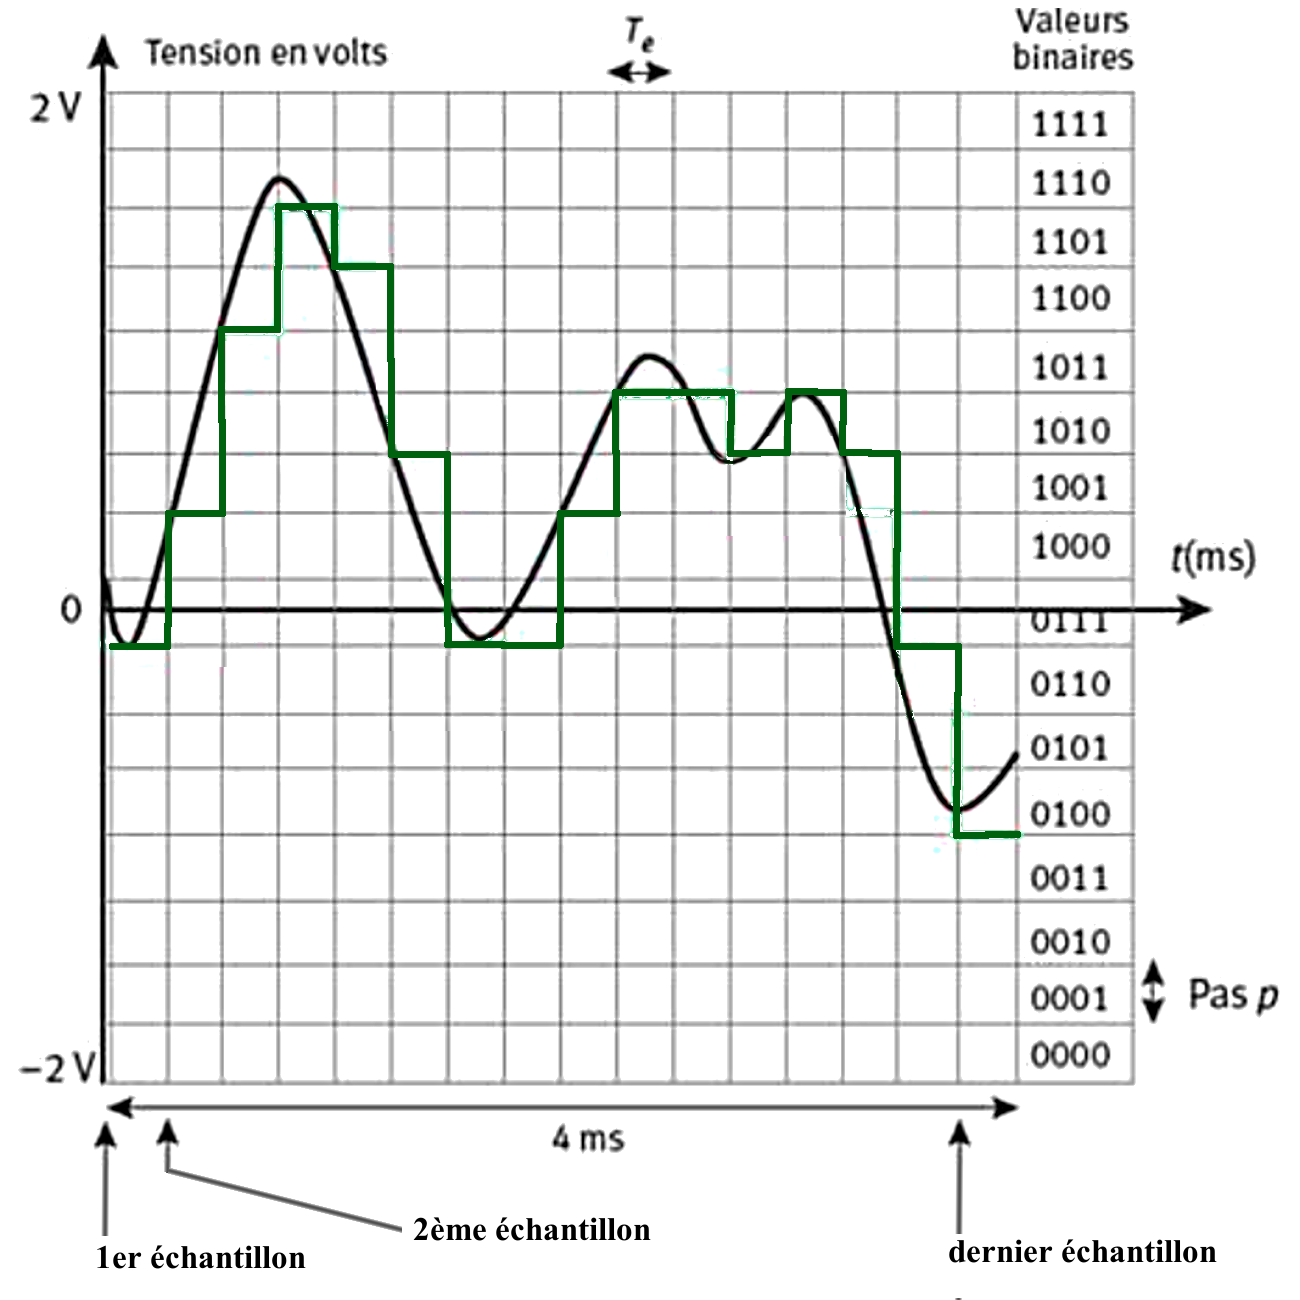
\includegraphics[width=0.70\textwidth]{images/conversion-AN.png}
    \caption{Conversion analogique-numérique}
    \label{fig:conversionANNA}
\end{figure}










\subsection{Quels sont les différents paramètres de conversion ?}





L’objectif de la numérisation est de transformer le signal analogique qui contient une quantité infinie d'amplitudes en un signal numérique contenant lui une quantité finie de valeurs. Alors le passage de l'analogique au numérique consiste en 2 étapes successives : l'échantillonnage et la conversion analogique-numérique (CAN).

\begin{figure}[H]
    \centering
    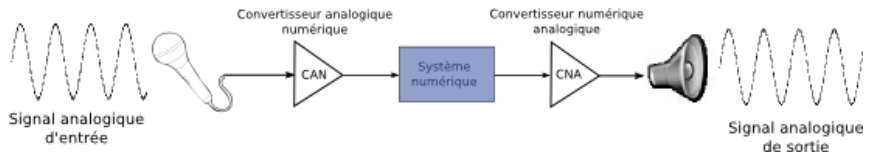
\includegraphics[width=0.95\textwidth]{images/parametres-conversion.PNG}
    \caption{Dispositif d'enregistrement numérique d'un son}
    \label{}
\end{figure}

L’échantillonnage est ce qui compose le signal analogique numérique. Le nombre d'échantillons composant le signal numérique devra être suffisamment grand pour pouvoir représenter le signal analogique de départ mais pas trop grand non plus pour ne pas être trop volumineux.

Pour ce faire, deux facteurs devront être ajustés pour répondre à ce cahier des charges : la précision et la rapidité.

Alors, le premier paramètre à fixer est la vitesse à laquelle seront prélevés les échantillons pour que la reconstruction du signal de sortie soit fidèle au signal d'entrée. La fréquence d'échantillonnage doit être suffisamment grande. En effet, si celle-ci est trop faible, les variations rapides du signal ne pourront être retranscrites.










\subsection{Que dois-je utiliser comme convertisseur AN pour équiper une bascule de poids lourds pour peser un camion de 80 tonnes (max) avec une précision de 10 kg ?}





\subsubsection{Type}

Ici le plus approprié serait le convertisseur à approximations successives étant donné qu'une balance doit donner une certaine valeur avant de donner la plus exacte et aussi car on va travailler par tranche de 10 kg.

Donc il n'est pas nécessaire d'avoir une valeur exacte 





\subsubsection{Résolution}  

$$ \frac{8000}{10} = 8000 $$

Étant donné que l'on veut une précision de 10 kg pour 80 Tonnes maximum, il nous faut assez de bits pour 8000 valeurs. 

$$ 2^{13} = 8192 $$

On aura donc besoin d'un convertisseur à 13 bits ! 

Si on prends un convertisseur 5 V. Notre calcul pour la résolution serait :

$$ \frac{ (5 - 0) }{ 2^{13} } = 0,0006103 $$

Soit, un peu plus de 0,610 mV.










\subsection{Quelle est la fréquence d’échantillonnage minimale pour la parole et la musique ?}






On nous dit que d'après "le théorème de NyquistShannon, une transmission sans perte d’information d’un signal ne pourra se faire que si sa fréquence est inférieure ou égale à la moitié de la fréquence d’échantillonnage". 

Ce qui veut dire que pour la musique la fréquence d'échantillonage sera de 40kHz et pour la parole 14 kHz.










\subsection{Comment et pourquoi utiliser un convertisseur pour réaliser un amplificateur audio en classe D, et pourquoi en classe D (et pas A, B ou AB) ?}





Les amplificateurs de classe D sont plus petits que les autres amplificateurs, ils dissipent moins de chaleur et ont un rendement plus élevés que les autres amplificateurs. L'amplificateur de classe D fonctionne grâce au principe de la modulation de largeur d'impulsion et c'est pour ça qu'il consomme moins d'énergie que les autres filtres. Nous avons ajouté une illustration d'un signal de sortie d'un amplificateur de classe D sur la figure \ref{fig:ampliD}.

\begin{figure}[H]
    \centering
    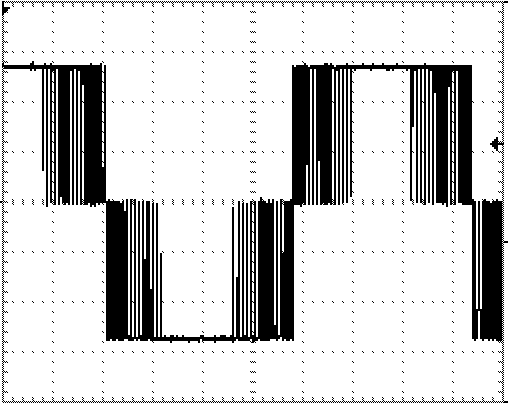
\includegraphics[width=0.5\textwidth]{images/PWM-signal.png}
    \caption{Signal de sortie d'un amplificateur de classe D}
    \label{fig:ampliD}
\end{figure}













\section{Conclusion}





Lors de la réalisation de ce rapport, nous avons appris ce qu’étaient les convertisseurs CAN et CNA. De plus, nous avons vu comment et lequel était le plus adapté en fonction d’une situation donnée, des performances de chacun, de son coût, ...

Mais aussi, quel convertisseur est utilisé en classe D et pourquoi ne pas utiliser ce convertisseur pour d’autres classes (A, B, AB).

Nous avons également appris à déterminer la fréquence d’échantillonnage, et à faire en sorte qu’elle soit adaptée au convertisseur choisi.

Nous sommes maintenant capables d’expliquer et de comprendre les choix fais lors d’une conversion AN ou NA.














\newpage \tableofcontents \listoffigures
\begin{thebibliography}{9}
\bibitem{1} https://sti2d.ecolelamache.org/iii\_conversion\_analogiquenumrique.html
\bibitem{2} https://fr.wikipedia.org/wiki/Convertisseur\_analogique-num\%C3\%A9rique
\bibitem{3} https://www.digikey.be/fr/articles/simplify-portable-low-power-audio-circuit-design-class-d-amplifiers
\bibitem{4} https://fr.wikipedia.org/wiki/Classes\_de\_fonctionnement\_d\%27un\_amplificateur\_\%C3\%A9lectronique\#Classe\_D
% \bibitem{5} 
% \bibitem{6} 
% \bibitem{7} 
% \bibitem{8} 
\end{thebibliography}




















\end{document}
